\documentclass[conference]{IEEEtran}
\IEEEoverridecommandlockouts
% The preceding line is only needed to identify funding in the first footnote. If that is unneeded, please comment it out.
\usepackage{cite}
\usepackage{amsmath,amssymb,amsfonts}
\usepackage{algorithmic}
\usepackage{graphicx}
\usepackage{textcomp}
\usepackage{xcolor}
\def\BibTeX{{\rm B\kern-.05em{\sc i\kern-.025em b}\kern-.08em
    T\kern-.1667em\lower.7ex\hbox{E}\kern-.125emX}}
\begin{document}

\title{IEEE Bigdata Cup 2018 FEMH Challenge Report\\
}

\author{\IEEEauthorblockN{1\textsuperscript{st} Soumya Ray}
\IEEEauthorblockA{\textit{Department of Electrical Engineering and Computer Science} \\
\textit{Case Western Reserve University}\\
Cleveland, Ohio, United States \\
sray@case.edu}
\and
\IEEEauthorblockN{2\textsuperscript{nd} Mingxuan Ju}
\IEEEauthorblockA{\textit{Department of Electrical Engineering and Computer Science} \\
	\textit{Case Western Reserve University}\\
	Cleveland, Ohio, United States \\
	mxj255@case.edu}
\and
\IEEEauthorblockN{3\textsuperscript{rd} Zhengkai Jiang}
\IEEEauthorblockA{\textit{Department of Electrical Engineering and Computer Science} \\
	\textit{Case Western Reserve University}\\
	Cleveland, Ohio, United States \\
	zxj89@case.edu }
\and
\IEEEauthorblockN{4\textsuperscript{th} Yufan Chen}
\IEEEauthorblockA{\textit{Department of Electrical Engineering and Computer Science} \\
	\textit{Case Western Reserve University}\\
	Cleveland, Ohio, United States \\
	yxc775@case.edu }
}

\maketitle

\section{Introduction}

\section{Methodology}
\subsection{Data Preprocessing:}
\begin{itemize}
	\item Silence and Noise Removal\\
	Doing a spot check on both training and testing set, we discovered that there exists silence or noise at the beginning of most audio files. We removed those silence or noise parts by calculating the average loudness of each audio file, and recursively comparing the value of 30\% of average loudness to first $\frac{3}{4}$ of the audio file.\\
	\item Equalizing Loudness:\\
	We also figured out that ,between training set and testing sets, there is a loudness difference not representative of class label. So, we linearly equalized average loudness of each file by the average loudness of all audio files. \\
\end{itemize}
\subsection{Feature Extraction:}
	We utilized general audio features: Zero Crossing Rae, Energy, Entropy of Energy, Spectral Centroid, Spectral Entropy, Spectral Spread, Spectral Entropy, Spectral Flux, Spectral Rolloff,  MFCCs, Chroma Vector and Chroma Deviation. The library we used for those feature extractions are pyAudioAnalysis\cite{b1}.\\
	After analyzing the dataset, we also noticed that number of local minimum amplitude peaks is one representative feature and we added that to feature list.\\
\subsection{Model Selection:}
	Our whole model-building infrastructure is based on scikit-learn\cite{b2}\cite{b3}. \\
	We tried K-Nearest Neighbor, Support Vector Machine, Boosting, Random Forest, Extratrees, Multiple Instance Learning, Label Propagation. After few experiments, it seemed like tree algorithms performed poorly on this task and we finalized our focus on SVM, Label Propagation, SVC and MILR with pipeline. This classifier undercalled Normal and Neoplasm patients, which we think is resulted from different class distributions between training and testing set. So, we converted this relatively complex learning task into three less complicated tasks: Normal vs. Pathological, Vocal vs. Rest of Diseases, and Phonotrauma vs. Neoplasm.[Fig. 1.] The reason why we design the pipeline this way is based on the difficulty of classification. (From easiest Normal vs. Pathological to hardest Phonotrauma vs. Neoplasm)
	\begin{figure}[htbp]
		\begin{center}
			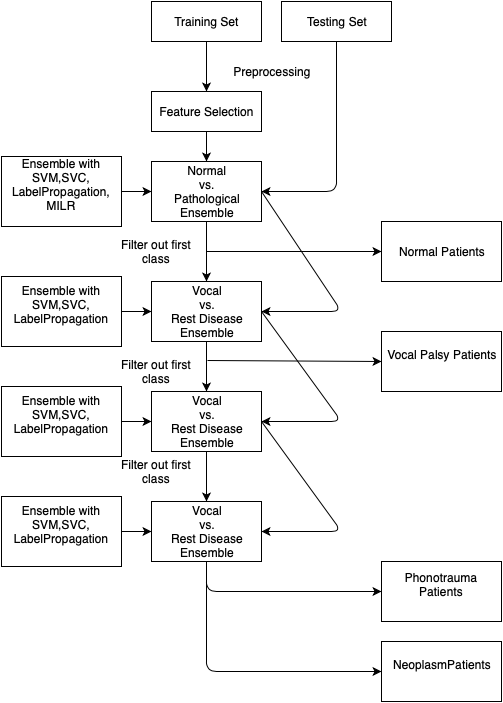
\includegraphics[scale=0.35]{Diagram_1.png}
		\end{center}
		\caption{Pipeline Ensemble}
	\end{figure}
	\subsection{Hyper Parameter Tuning:}
		Since the size of training set is getting smaller and smaller as we propagate through the pipeline, in order to get trustworthy accuracy to tune parameter for SVC, for all three ensembles, we use the same parameter tuned in the first ensemble. The process is pretty straightforward; we simply set up two loops, one of which for C and one of which for gamma. The tuned parameters are 10 for C, and 0.01 for gamma. Also due to the skewed distribution in training set, we modify the class weight with respect to the proportion of class. 


\section{Results \& Discussion}

We have submitted several sets of results. It seems that it is difficult to detect the normal cases. While our model are able to detect the normal examples with 70.0\% to 80.0\% in Augut's submission, the prediction is pretty bad. 

\begin{table}[htbp]
	\caption{July's cross validation}
	\begin{center}
		\begin{tabular}{|c|c|}
			\hline
			Model & Accuracy \\
			\hline
			K-Nearest Neighbor & 68.0 \% \\
			\hline
		\end{tabular}
		\label{tab0}
	\end{center}
\end{table}

\begin{table}[htbp]
	\caption{August's cross validation}
	\begin{center}
		\begin{tabular}{|c|c|c|}
			\hline
			Model & Support Vector Machine & Random Forest \\
			\hline
			normal accuracy & 72.0 \% & 77.0 \% \\
			\hline
			vocal palsy & c & c \\
			\hline
			phonotrauma & c & c \\
			\hline
			Neoplasm &c & c\\
			\hline
		\end{tabular}
		\label{tab1}
	\end{center}
\end{table}

\begin{table}[htbp]
	\caption{October's Cross Validation}
	\begin{center}
		\begin{tabular}{|c|c|}
			\hline
			Model & Support Vector Machine \\
			\hline
			Normal & 87.0 \% \\
			\hline
			Volcal palsy & 89.0 \% \\
			\hline
			Phonotrauma & 74.0 \% \\
			\hline
		\end{tabular}
		\label{tab2}
	\end{center}
\end{table}



\begin{table}[htbp]
	\caption{Results}
	\begin{center}
		\begin{tabular}{|c|c|c|c|}
			\hline
			Attempt & Sensitivity & Specificity & UAR \\ 
			\hline
			July & 83.7 \% & 56.0 \% & 51.83 \% \\
			\hline
			August & 95.1 \% &  32.0 \% & 58.4 \% \\  
			\hline
			October & 82.2 \% & 60.0 \% & 63.77\% \\
			\hline
		\end{tabular}
		\label{tab3}
	\end{center}
\end{table}
		

\begin{thebibliography}{00}
\bibitem{b1} Tyiannak, pyAudioAnalysis, https://github.com/tyiannak/pyAudioAnalysis/wiki/3.-Feature-Extraction
\bibitem{b2} Fabian Pedregosa, Gaël Varoquaux, Alexandre Gramfort, Vincent Michel, Bertrand Thirion, Olivier Grisel, Mathieu Blondel, Peter Prettenhofer, Ron Weiss, Vincent Dubourg, Jake Vanderplas, Alexandre Passos, David Cournapeau, Matthieu Brucher, Matthieu Perrot, Édouard Duchesnay, Scikit-learn: Machine Learning in Python
\bibitem{b3} Lars Buitinck1, Gilles Louppe2, Mathieu Blondel3, Fabian Pedregosa4, Andreas C. Mu ̈ller5, Olivier Grisel6, Vlad Niculae7, Peter Prettenhofer8, Alexandre Gramfort4,9, Jaques Grobler4, Robert Layton10, Jake Vanderplas11, Arnaud Joly2, Brian Holt12, and Ga ̈el Varoquaux4, API design for machine learning software: experiences from the scikit-learn project
\end{thebibliography}
\end{document}
